Entre os muitos desafios enfrentados pelos agricultores, a deficiência de minerais nas plantas é uma preocupação significativa, pois pode resultar em perdas de produtividade e qualidade dos cultivos. A mexerica (Citrus reticulata) é uma das culturas suscetíveis a deficiências minerais, o que pode afetar seu crescimento, desenvolvimento e produção.

O artigo de \textcite{EstadoArte1} discute avanços recentes nas tecnologias de visão computacional, aprendizado de máquina (ML) e aprendizado profundo (DL), que têm sido aplicadas ao monitoramento agrícola para melhorar a produtividade e a qualidade das colheitas. Entre as tecnologias abordadas, destacam-se imagens de satélite, sensoriamento remoto, Internet das Coisas (IoT), dispositivos de sensor e Veículos Aéreos Não Tripulados (VANTs). Esses sistemas são utilizados para capturar dados visuais e detectar deficiências nutricionais em tempo real, permitindo um diagnóstico precoce e aumentando a eficiência na aplicação de insumos agrícolas.

O artigo cita trabalhos que demonstram como a visão computacional, combinada com ML e DL, pode identificar padrões visuais como coloração, textura e bordas em imagens de plantas. Esse exemplo ilustra como essas técnicas permitem um diagnóstico não invasivo, usando câmeras digitais e algoritmos avançados para diferenciar entre folhas saudáveis e folhas com deficiência nutricional.

Com base nesses avanços, é viável que o projeto NitrusLeaf implemente um sistema semelhante, utilizando smartphones e visão computacional para capturar e analisar imagens de folhas de mexerica. Com o suporte de algoritmos de ML/DL, o sistema pode processar essas imagens para identificar deficiências específicas, como de cobre e manganês, diretamente no campo.

O artigo de \cite{EstadoArte2} explora um pipeline detalhado \Cref{fig:pipeline} para identificar doenças e deficiências nutricionais em plantas, baseado em técnicas de processamento de imagem. Esse pipeline, ou sequência organizada de etapas, permite a análise automatizada e eficiente de imagens de plantas, produzindo diagnósticos agrícolas precisos. O pipeline descrito no artigo inclui as seguintes fases: Aquisição de imagem, Pré-processamento, Segmentação, Extração de características, Classificação e, finalmente, Detecção e Diagnóstico. Cada fase depende da anterior e contribui para refinar e analisar os dados, de modo a produzir uma resposta confiável sobre a condição da planta.

\begin{itemize} 
    \item \textbf{Aquisição de imagem}: Envolve a captura de imagens de plantas utilizando câmeras, drones (Veículos Aéreos Não Tripulados - VANTs) ou dispositivos móveis. Essa etapa assegura que as imagens tenham qualidade suficiente para as fases subsequentes do processamento.
    \item \textbf{Pré-processamento}: Aqui, técnicas de correção de ruído, ajuste de contraste e brilho, além de redimensionamento e rotação, são aplicadas para melhorar a qualidade da imagem e facilitar a segmentação. 
    \item \textbf{Segmentação de imagem}: É feita para isolar a folha ou parte relevante da planta, separando-a do fundo. Técnicas comuns incluem limiarização, segmentação por cor e abordagens de aprendizado de máquina. \item \textbf{Extração de características}: Essa etapa analisa e extrai informações importantes, como cor, textura e forma, que são essenciais para diferenciar entre folhas saudáveis e afetadas. Métodos como histogramas de cor e a Matriz de Co-ocorrência de Níveis de Cinza (GLCM) são comumente usados. 
    \item \textbf{Classificação}: Modelos de aprendizado de máquina ou redes neurais profundas (como CNNs e SVMs) são empregados para classificar as imagens, diferenciando as folhas saudáveis das que apresentam deficiências ou doenças. 
    \item \textbf{Detecção e Diagnóstico}: A última etapa envolve o diagnóstico da condição da planta, onde é identificada a doença ou deficiência nutricional específica, e recomendações são geradas com base nos resultados da classificação.
\end{itemize}

\begin{figure}[H]
    \centering
    \caption{Esquema do pipeline para detecção de doenças em plantas baseada em imagens}
    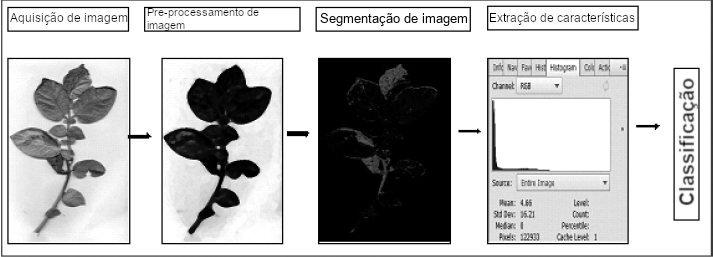
\includegraphics[width=0.8\linewidth]{Illustrations/pipeline.png}
    \label{fig:pipeline}
    \SourceOrNote{Adaptado de \cite{EstadoArte2}}
    \end{figure}


    Além disso, o artigo explora técnicas não intrusivas para a detecção de deficiências nutricionais, utilizando métodos avançados de análise de imagens. Por exemplo, uma tabela destaca o uso do sistema de cores RGB (Red, Green, Blue) para identificar deficiências de nutrientes, incluindo a deficiência de manganês em citrus. Essa abordagem reforça a viabilidade do projeto NitrusLeaf, que tem como objetivo identificar deficiências de cobre e manganês nas folhas de mexerica. Ao adotar essas tecnologias e adaptar o pipeline descrito, o NitrusLeaf poderá se consolidar como uma solução eficaz e prática para diagnósticos agrícolas baseados em visão computacional.



O artigo de \textcite{EstadoArte3} utiliza os modelos Inception-ResNet v2, Autoencoder de Rede Neural Convolucional (CNN), e uma combinação desses dois modelos por meio de Ensemble Averaging para melhorar a detecção precoce de deficiências nutricionais de cálcio, nitrogênio e potássio em plantações de tomate. A identificação rápida dessas deficiências é essencial, pois a falta de intervenção pode levar a condições mais graves, incluindo doenças que afetam a produtividade e a saúde das plantas. Para garantir que os modelos fossem treinados com imagens robustas e representativas, os autores aplicaram técnicas de pré-processamento e aumento de dados (data augmentation), como ajuste de ângulo, brilho e contraste. Essas técnicas aumentaram a diversidade visual do conjunto de dados, ajudando os modelos a generalizar melhor e a detectar padrões de deficiência com mais precisão.

A escolha dos modelos Inception-ResNet v2 e Autoencoder foi motivada pela capacidade dessas arquiteturas em capturar características visuais complexas nas folhas e nos frutos, essenciais para distinguir entre deficiências nutricionais que compartilham sintomas visuais semelhantes. O Inception-ResNet v2, por exemplo, combina as vantagens das redes Inception e ResNet, permitindo uma análise detalhada de padrões locais e globais na imagem. Já o Autoencoder oferece uma estrutura de compressão e reconstrução útil para destacar anomalias visuais, como as causadas por deficiências. O estudo usou um conjunto de 571 imagens de tomates cultivados em estufas, das quais 80\% (461 imagens) foram destinadas ao treinamento e 20\% (110 imagens) para a validação dos modelos. Após extensivos testes, os resultados mostraram que o Inception-ResNet v2 obteve uma precisão de 87,27\%, o Autoencoder alcançou 79,09\%, e a técnica de Ensemble Averaging conseguiu uma precisão de 91\%.

As abordagens e metodologias deste artigo são relevantes para nosso projeto, pois ambos compartilham o foco em visão computacional e aprendizado profundo para a detecção de deficiências nutricionais em plantas. Enquanto o artigo de Tran et al. se concentra em deficiências de nitrogênio e potássio em folhas de tomate, nosso projeto utiliza técnicas similares para identificar deficiências de cobre e manganês em folhas de mexerica. Assim, este trabalho oferece uma base metodológica útil, especialmente na escolha de modelos de CNN e na importância de uma abordagem de ensemble para melhorar a precisão no diagnóstico.

Esses resultados indicam que, com o uso apropriado das tecnologias discutidas, nosso projeto NitrusLeaf poderá alcançar resultados satisfatórios. Aproveitando as tecnologias descritas, buscamos oferecer uma funcionalidade avançada ao sistema, permitindo a identificação precisa de deficiências minerais, como as de manganês e cobre, por meio da análise de imagens capturadas pelos usuários.